\section{Aufbau}
\label{sec:Aufbau}
Gemäß Abbildung \ref{fig:HVD} wird die Glühkathode an eine Konstantstromquelle angeschlossen. Zwischen Kathode und Anode wird eine $0\si{\volt}$ und $260\si{\volt}$ regulierbare Spannungsquelle mit eingebautem Ampere-Meter angeschlossen.
Für die Messung des Anlaufstroms im Bereich $V<0$ wird wie in Abbildung \ref{fig:aufbau} zu sehen ein empfindlicheres $\si{\nano\ampere}$-Meter angeschlossen und eine zwischen $0\si{\volt}$ und $1\si{\volt}$ regulierbare Spannungsquelle verwendet.
\begin{figure}
\centering
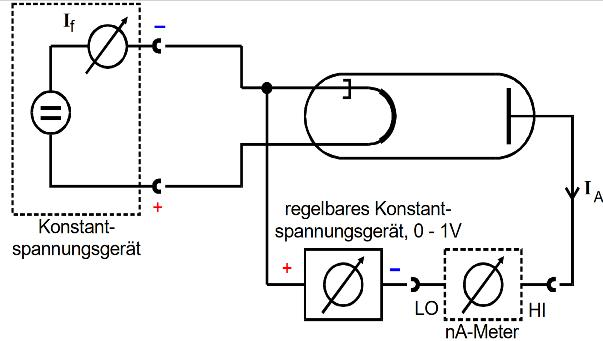
\includegraphics[width=\linewidth-70pt,height=\textheight-70pt,keepaspectratio]{content/images/aufbau.jpg}
\caption{Aufbau zur Messung des Anlaufstroms einer Hochvakuumdiode\cite{V504}}
\label{fig:aufbau}
\end{figure}